\documentclass[11pt,a4paper, twocolumn]{article}
\usepackage[T1]{fontenc}
\usepackage[utf8]{inputenc} % para poder usar tildes en archivos UTF-8
\usepackage[spanish]{babel} % para que comandos como \today den el resultado en castellano
\usepackage{a4wide} % márgenes un poco más anchos que lo usual
\usepackage[sinEntregas]{caratula}
\usepackage{float} 
\usepackage[section]{placeins}  
\usepackage{enumerate}

%\usepackage{helvet}

\begin{document}

\titulo{Trabajo Práctico 02}
\subtitulo{Informe}

\fecha{\today}

\materia{Laboratorio de Datos}
\grupo{EcuJaRu2}

\integrante{Fomina, Evangelina}{520/23}{evangelina.miloslav9@gmail.com}
\integrante{Niikado, Marina}{711/07}{niikadomarina@gmail.com}
\integrante{Borja, Kurt}{695/19}{kuurtb@gmail.com}
% Pongan cuantos integrantes quieran
\onecolumn

\maketitle

%\twocolumn

%\section{Resumen}
\section{Introducción}

El objetivo de este trabajo práctico es desarrollar dos modelos de clasificación de letras mayúsculas escritas a mano, uno para las letras ``A'' y ``L'' y otro para todas las vocales del alfabeto latino. Usando los métodos de aprendizaje automático supervisado \textbf{k-nearest neighbors} (\textbf{k-NN}) y \textbf{decision tree} respectivamente.

Para esto contamos con una versión reducida del popular dataset EMNIST (Cohen et al., 2017), que incluye solo las letras mayúsculas del alfabeto inglés. Viene dado como una matriz cuyas columnas representan el valor del canal alpha de cada pixel de una imagen de tamaño $28 \times 28$, junto con un label (785 columnas) y cuyas filas son cada elemento de la muestra. Este cuenta con 26 clases (una para cada letra) y una muestra de 2400 letras escritas a mano para cada clase, en total 62400 elementos balanceados.

A continuación, en lo que resta de la sección, los valores de los pixeles serán escalados con el método min-max.

\begin{figure}[H]
	\centering
	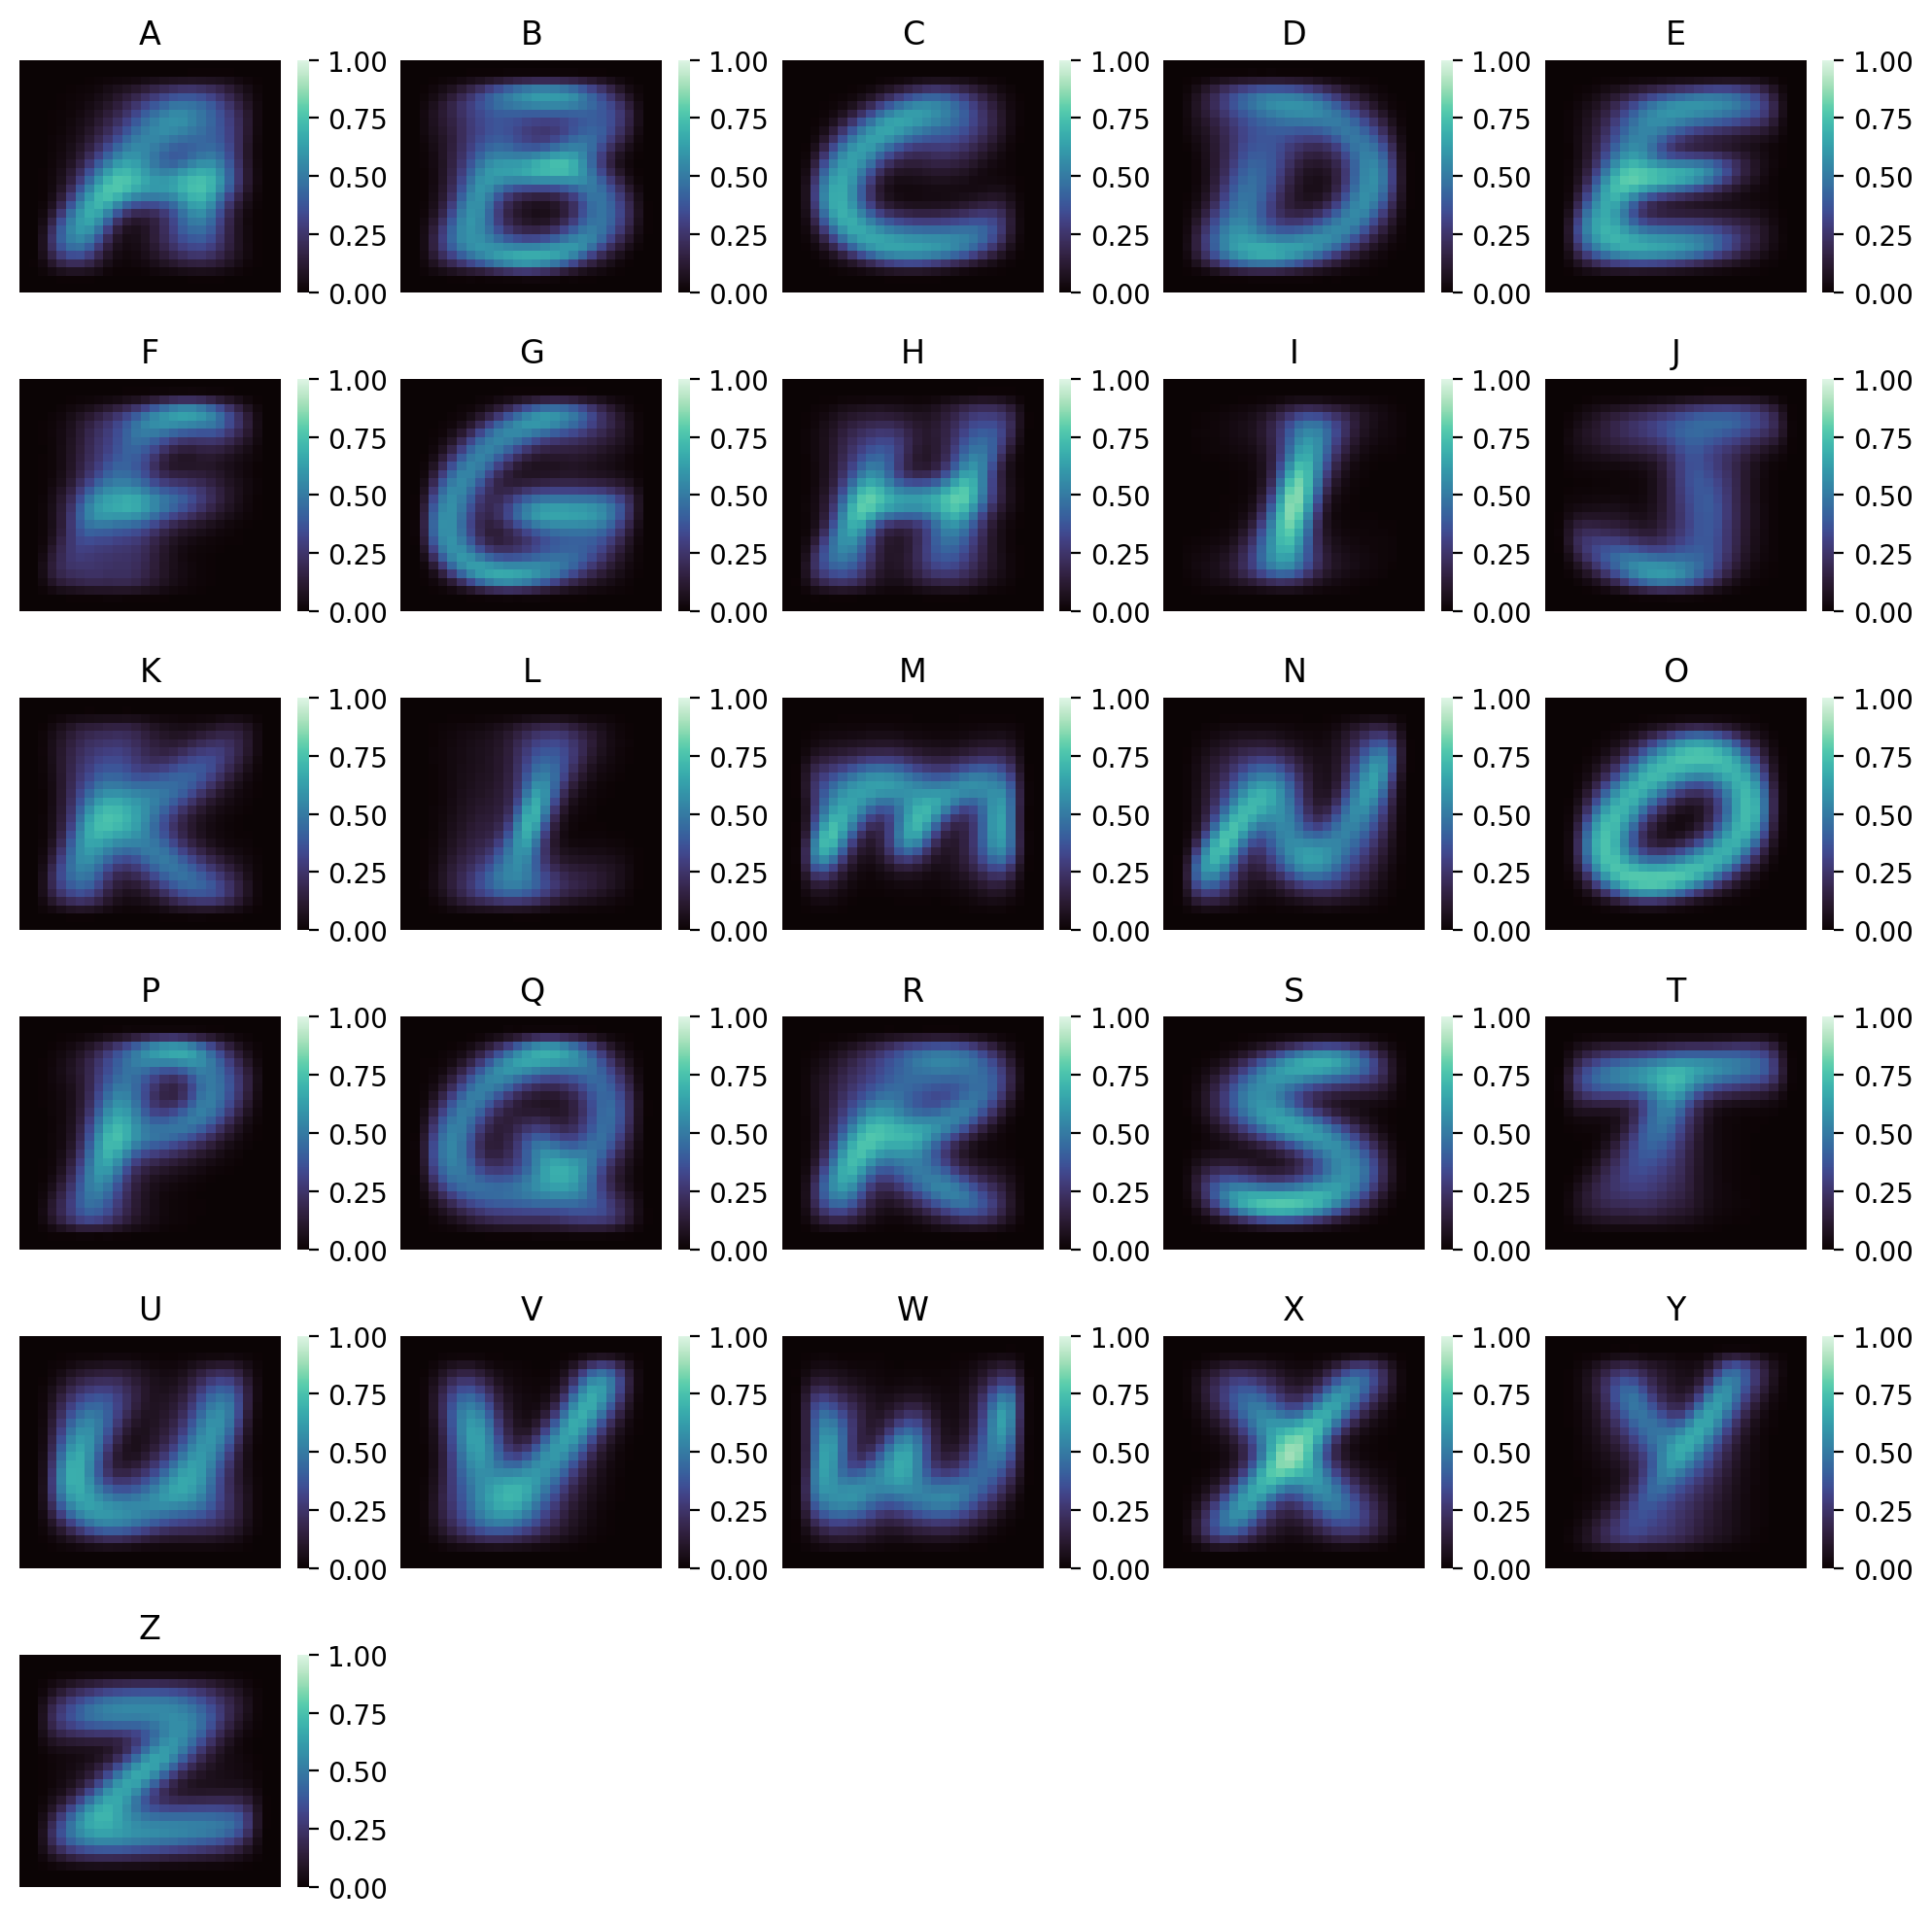
\includegraphics[scale=0.5]{figuras/1a.png}
	\caption{Media de cada parametro para cada clase.}
	\label{fig:1a}
\end{figure}

Con el proposito de reducir la complejidad de nuestros modelos, para seleccionar los atributos mas relevantes, tomamos la media de cada parametro por clase, como se observa en la Figura \ref{fig:1a}. Luego tomamos la desviación estandar de cada pixel de estas medias como se observa en la Figura \ref{fig:2a}.

\begin{figure}[H]

	\centering
	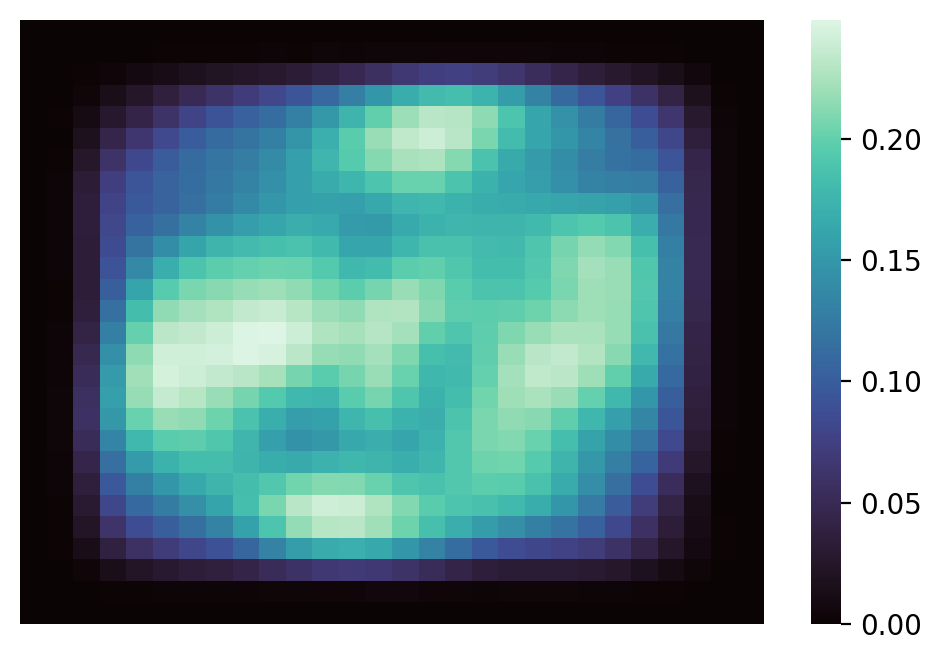
\includegraphics[scale=0.8]{figuras/2a.png}
	\caption{Desviación estandar entre la media de todas las clases.}
	\label{fig:2a}
\end{figure}

Nuestra hipótesis es que las variables con mas desviación estandar entre clases, codifican mas información sobre estas. Como nuestros modelos van a ser entrenados sobre un subconjunto de estas clases, tomamos las mas relevantes para nuestro objetivo, como se ve en la Figura \ref{fig:3a}.

\begin{figure}[H]
	\centering
	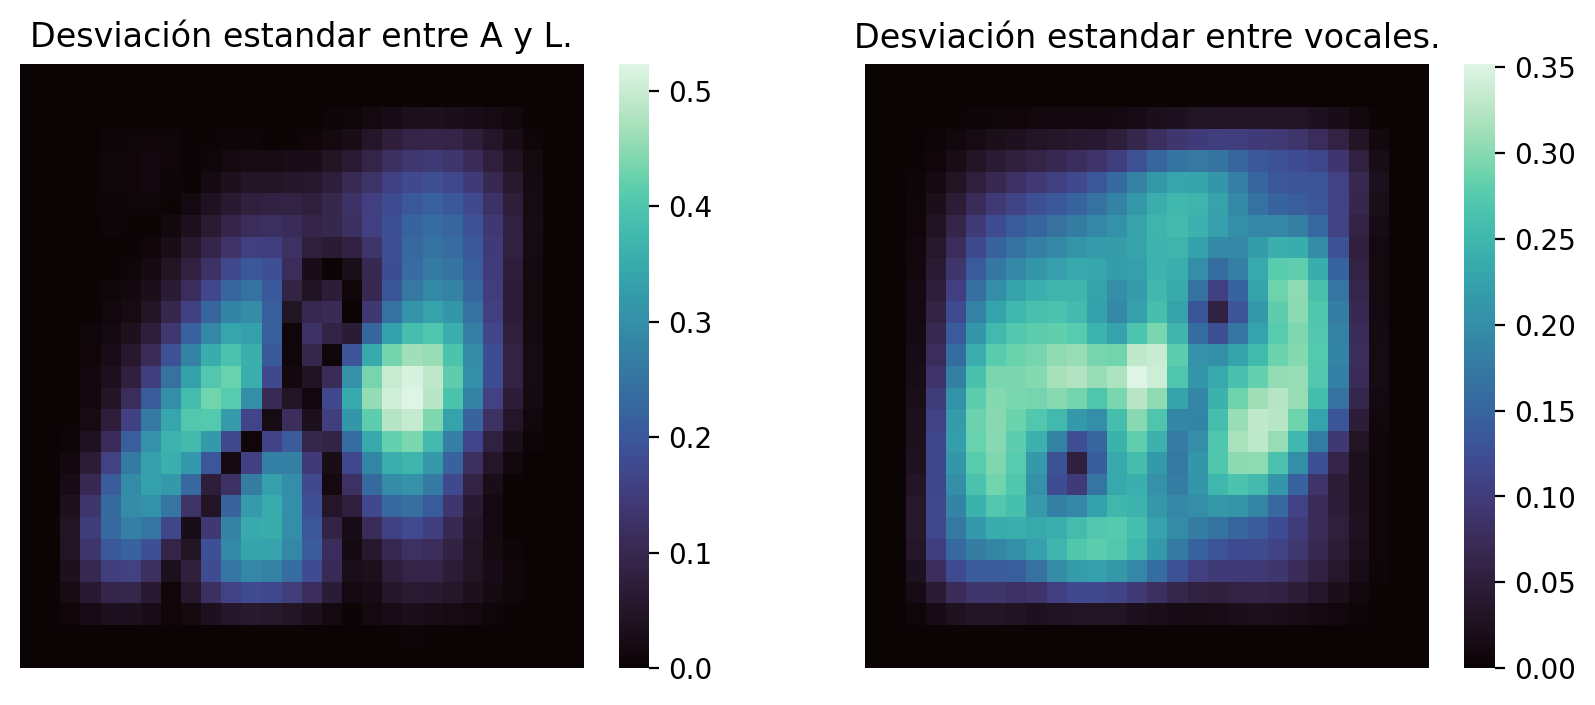
\includegraphics[scale=0.7]{figuras/3a.png}
	\caption{Desviación estandar entre la media de clases relevantes.}
	\label{fig:3a}
\end{figure}

Luego para analizar que tanto se parecen dos clases entre si tomamos el coeficiente de correlación de Pearson entre las medias de cada clase. Por ejemplo las letras ``E'' y ``L'' tienen un coeficiente de correlación de $\approx 0.64$ a comparación de las letras ``E'' y ``M'' que tienen un coeficiente de correlación de $\approx 0.41$. Estos resultados son intuitivos ya que las letras ``E'' y ``L'' comparten trazos. En la Figura \ref{fig:4a} vemos el coeficiente de correlación para todos los posibles pares de letras.

\begin{figure}[H]
	\centering
	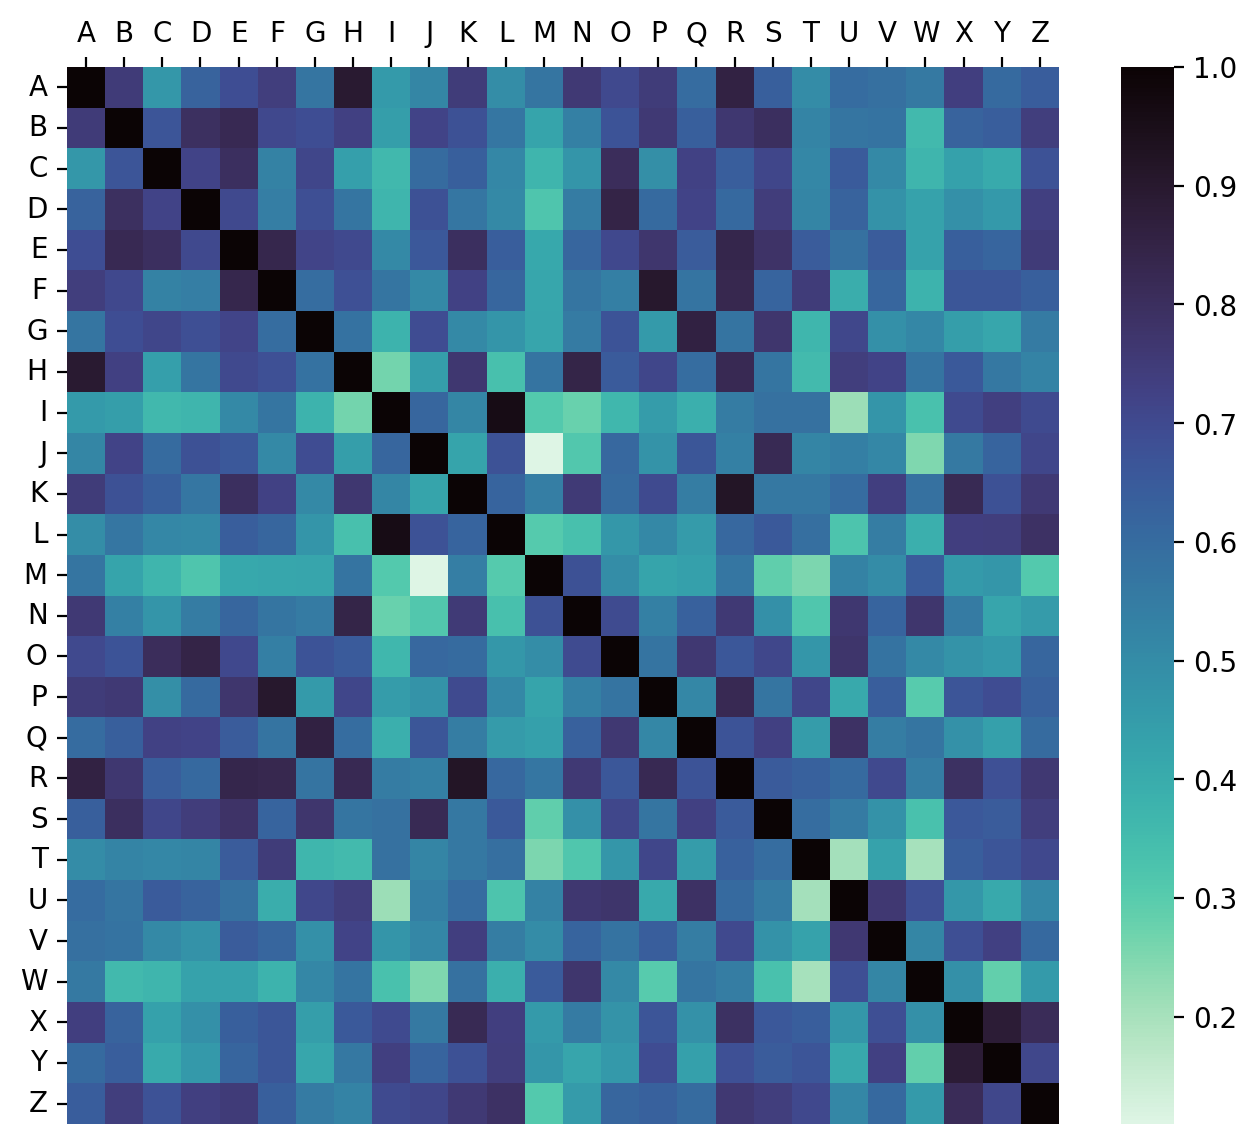
\includegraphics[scale=0.6]{figuras/4a.png}
	\caption{Coeficientes de correlación entre la media de cada clase.}
	\label{fig:4a}
\end{figure}

Por otro lado para analizar que tanto se parecen los elementos de una clase entre si, tomamos la media de la desviación estandar de cada pixel de esa clase. Por ejemplo en la Figura \ref{fig:5a} podemos ver la desviación estandar para la letra ``C'' su media es $\approx 0.20$.

\begin{figure}[H]
	\centering
	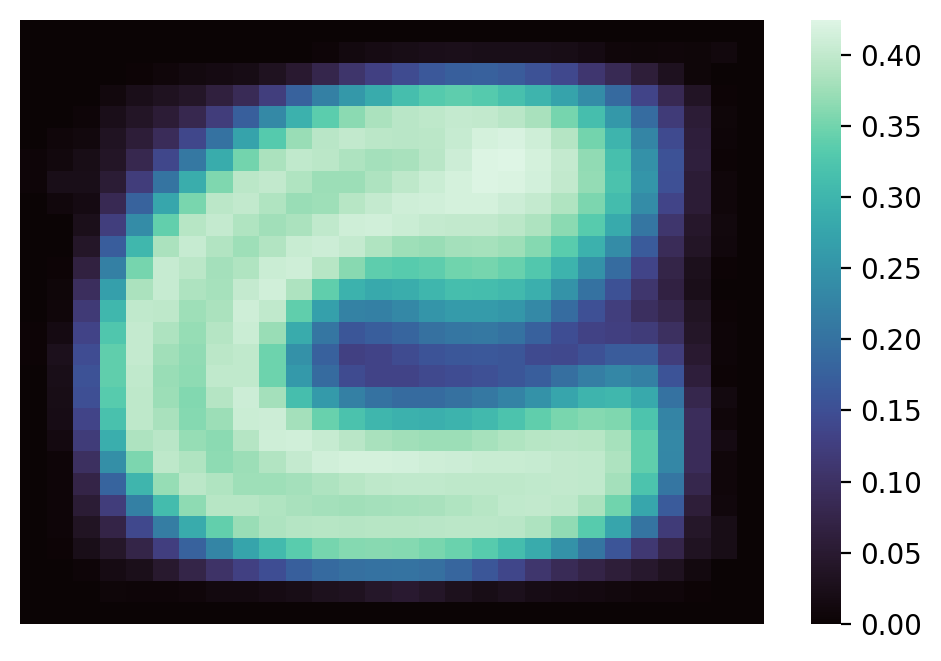
\includegraphics[scale=0.8]{figuras/5a.png}
	\caption{Desviación estandar de cada pixel de la letra C.}
	\label{fig:5a}
\end{figure}

Si realizamos este mismo proceso para cada letra obtenemos los resultados de la Figura \ref{fig:6a}

\begin{figure}[H]
	\centering
	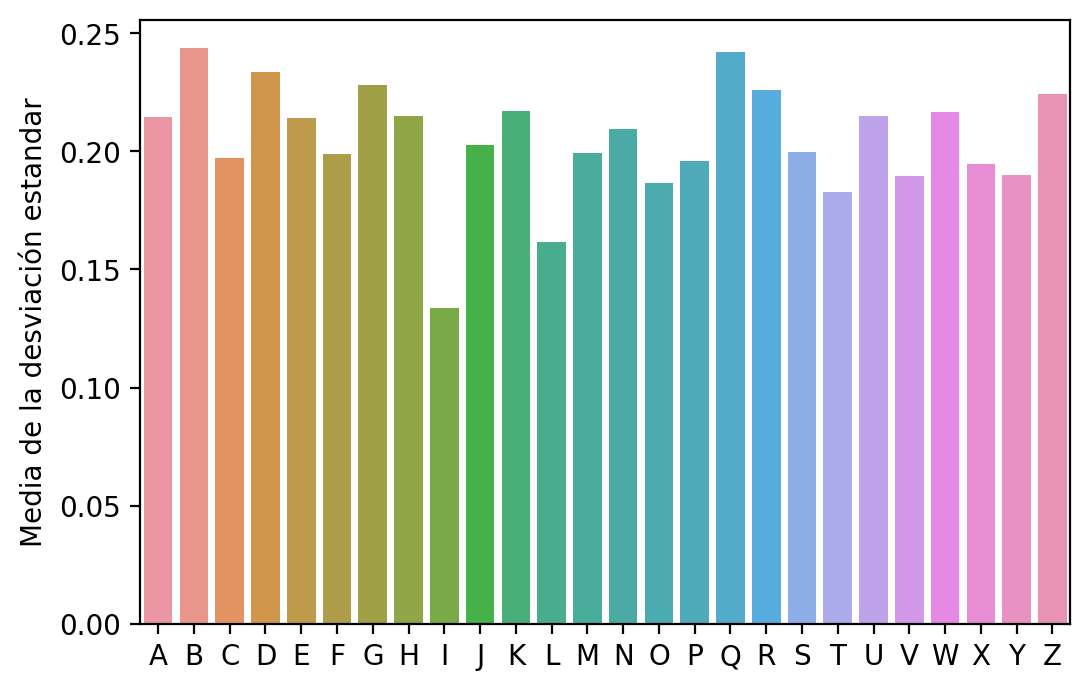
\includegraphics[scale=0.8]{figuras/6a.png}
	\caption{Media de la desviación estandar para cada letra.}
	\label{fig:6a}
\end{figure}

\section{Experimentos realizados}
\subsection{Clasificación binaria}
Para proceder con la tarea de clasificación binaria, fue necesario seleccionar solamente dos clases de todos los datos. Se seleccionaron las letras 'A' y 'L', como se pidió en la consigna.
Como el dataset que nos llegó está limpio, no hubo ningún obstaculo en conseguir que estén balanceadas las partes de datos de entrenamiento y de evaluación ('X train', 'X test'). 
\begin{itemize}
    \item[]
       \textbf{Experimento 1: Ajusto de un modelo de KNN eligiendo 3 atributos}

En este experimento se ajustó un modelo de K-Nearest Neighbors (KNN) en el valor de cantidad de vecino = 3. 
Para seleccionar los mejores 3 atributos se hizo un sample de 100 atributos 
\end{itemize}

\subsection{Clasificación multiclase}
Se cuenta con un modelo de árbol de decisión tal que, dada una imagen, predice a cuál de las vocales ('A', 'E', 'I', 'O', 'U') corresponde. El objetivo de los experimentos descriptos a continuación es seleccionar el mejor modelo que cumpla esta tarea. Para esto se generó un dataframe tomando sólo los datos correspondientes a las letras mencionadas y se los separó en un conjunto de datos de desarrollo (entrenamiento) y otro de validación (held-out). Para reducir el tiempo de ejecución de los experimentos, se tomaron solo los atributos (píxeles de la imagen) considerados más relevantes.

\begin{itemize}
	\item[]
		\textbf{Experimento 1: Ajuste de un modelo de Árbol de Decisión con distintas profundidades}

En este experimento se ajustó un modelo DecisionTreeClassifier variando la profundidad máxima del árbol (max\_depth) desde 1 hasta 21 con incrementos de 2. Se midió la performance del modelo en el conjunto de datos de desarrollo (X\_train).

\begin{figure}[H]
	\centering
	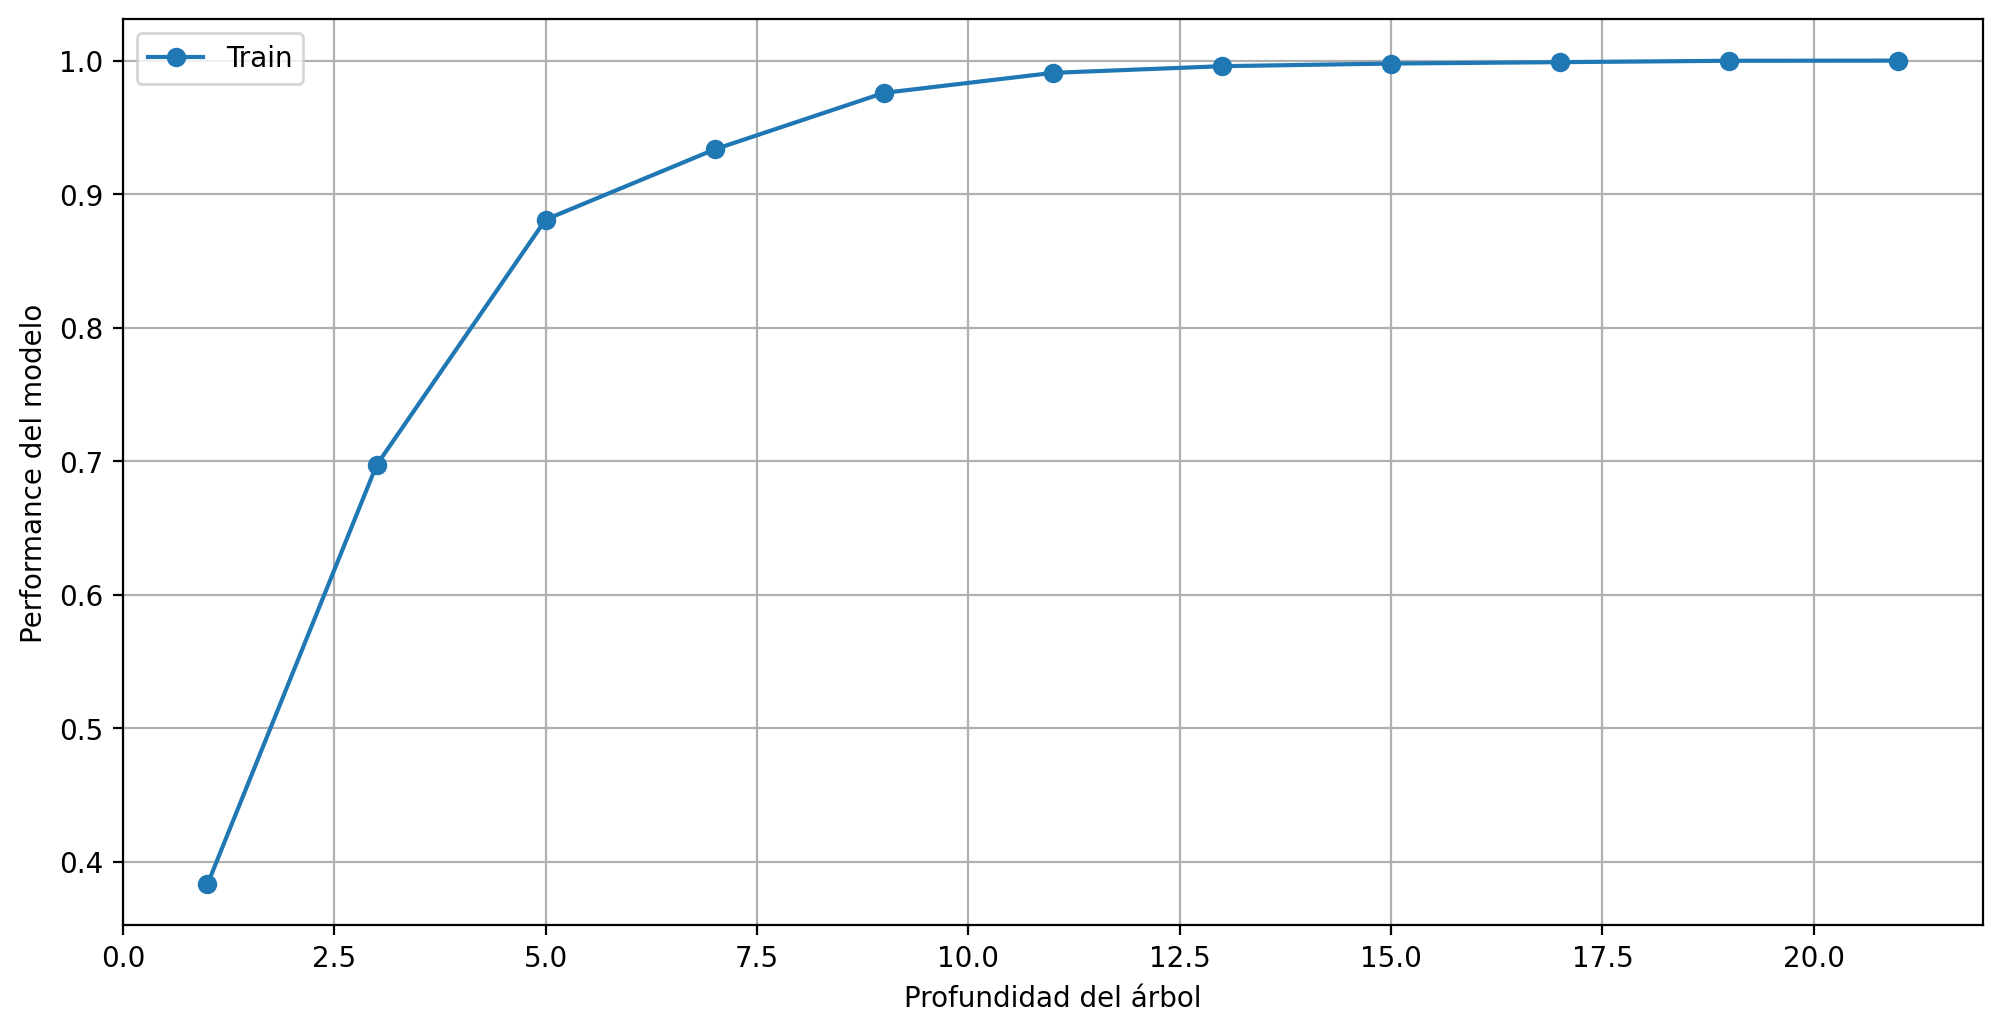
\includegraphics[scale=0.6]{figuras/3b.png}
	\caption{Performance vs profundidad del modelo de árbol de decisión}
	\label{fig:3b}
\end{figure}

Los resultados de este experimento, tal como se ve en la figura \ref{fig:3b}, mostraron que la precisión del modelo aumenta con la profundidad del árbol, lo cual es esperado. Sin embargo, es importante notar que profundidades mayores pueden llevar a sobreajuste (overfitting), donde el modelo aprende demasiado bien los datos de entrenamiento y pierde capacidad de generalización. 

	\item[]
		\textbf{Experimento 2: Validación Cruzada con K-Fold }
 
Con este experimento se busca encontrar la mejor configuración de hiperparámetros para el modelo. 

A partir del experimento anterior se pudo intuir que para encontrar la profundidad más adecuada, se podían descartar los valores muy bajos (1-6) para evitar el subajuste, y los demasiados altos (mayores a 14) para el sobreajuste. Por esto se optó por variar el hiperparámetro \textit{max\_depth} entre profundidades intermedias. 
Al mismo tiempo, se buscó variar el hiperparámetro \textit{criterion} para obtener la combinación óptima entre profundidad y criterio. 

Se utilizó validación cruzada con KFold (n\_splits=10, shuffle=True, random\_state=1) para evaluar el rendimiento de los modelos DecisionTreeClassifier, en el conjunto de datos de desarrollo (X\_train), con diferentes profundidades máximas del árbol (7 a 14) y criterios de elección de atributos (Gini y Entropy). Una vez obtenidos los distintos valores de performance, separados en datos de entrenamiento y test, por cada \textit{max\_depth} y a su vez, divididos por \textit{criterion}, se tomó el promedio de los scores de performance, resultando en el siguiente gráfico: 

\begin{figure}[H]
	\centering
	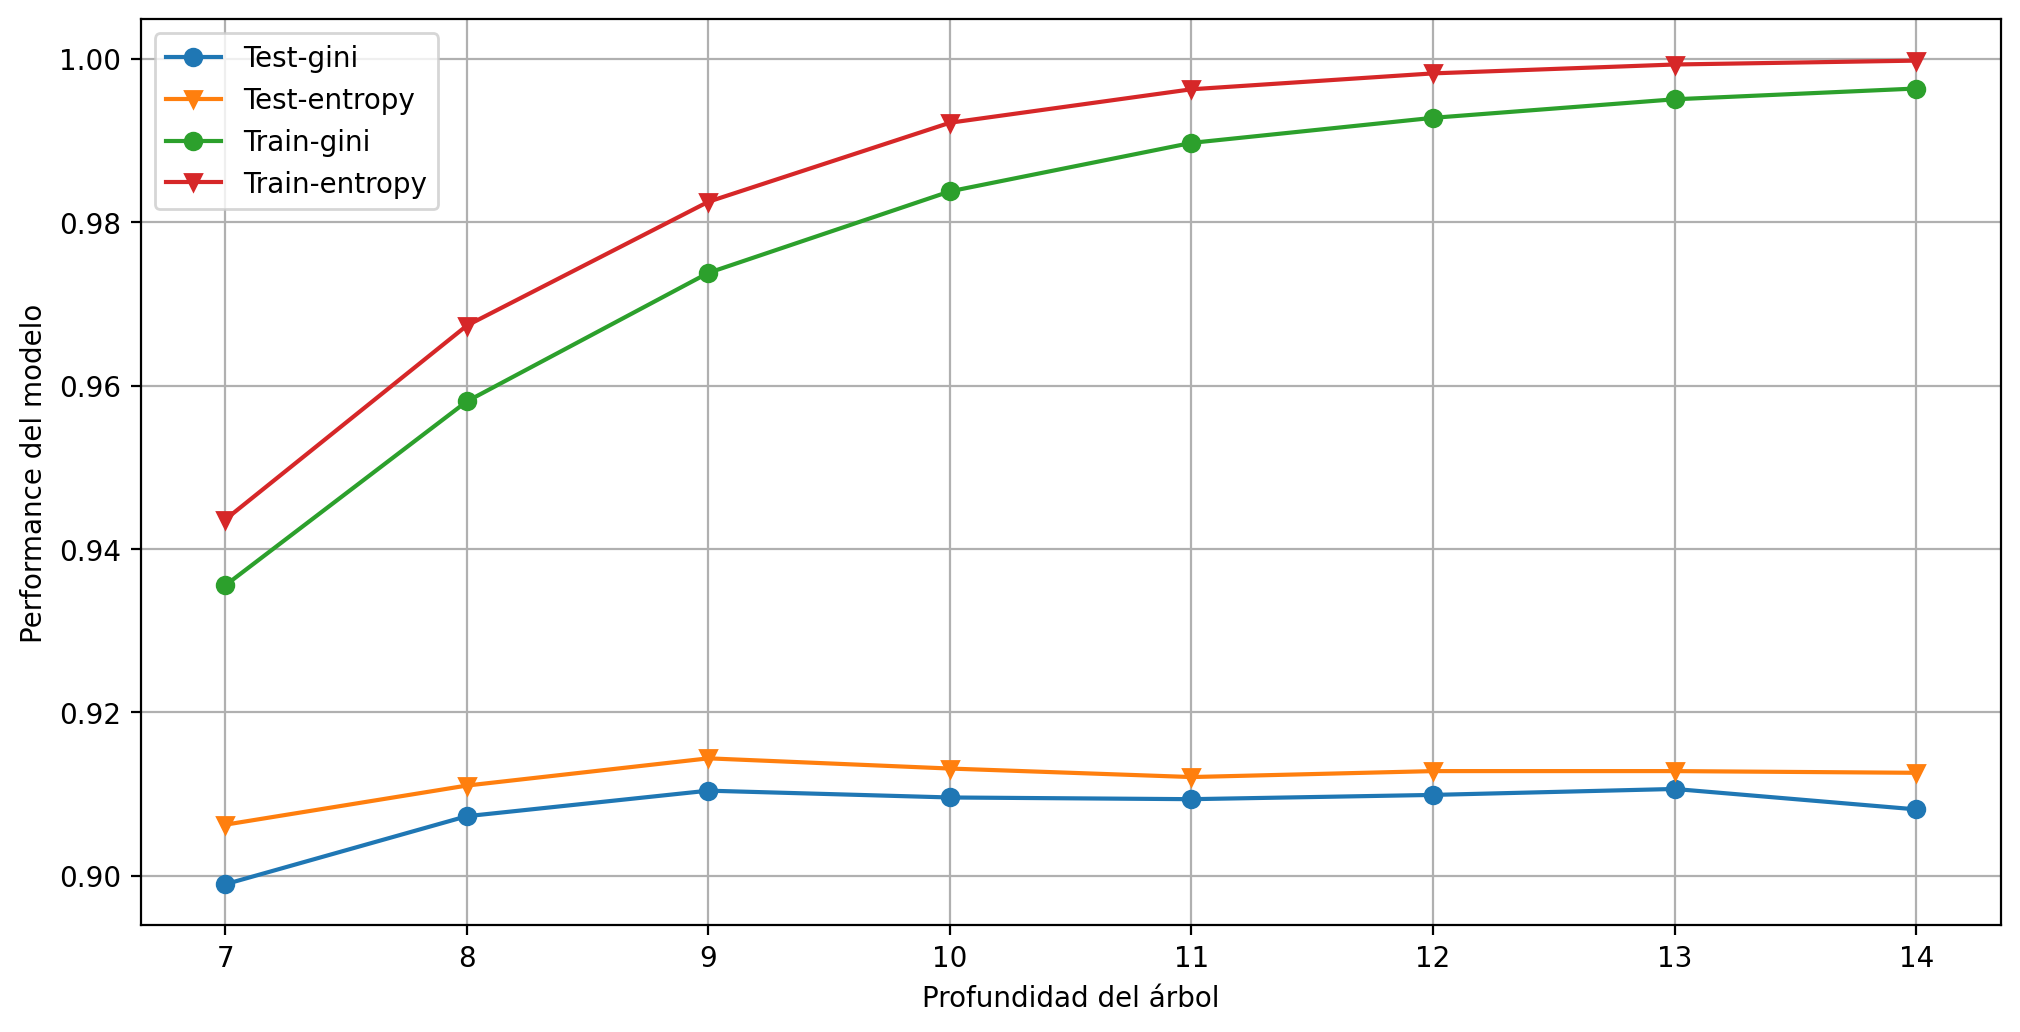
\includegraphics[scale=0.6]{figuras/3c.png}
	\caption{Performance vs profundidad del modelo de árbol de decisión para criterios Gini y Entropy separados en datos de Train y Test}
	\label{fig:3c}
\end{figure}

Como se puede observar en la figura \ref{fig:3c}, los valores de performance en los datos de entrenamiento (Train-gini, Train-entropy) se comportan de forma similar a lo visto en el Experimiento 1, aumentando la precisión del modelo a mayor profundidad del árbol. 
El comportamiento con los datos de test (Test-gini, Test-entropy), indica que la mayor precisión se obtiene con \textit{max\_depth} = 9. 
Con respecto al criterio de elección de atributos, en ambos conjuntos de datos, el más indicado parece ser \textit{criterion} = Entropy.

Según este experimento, la mejor combinación de hiperparámetros es con \textit{max\_depth} = 9 y \textit{criterion} = Entropy, obteniendo un promedio de performance de 0.914375.

	\item[]
		\textbf{Experimento 3: Entrenamiento y análisis de performance con el mejor modelo}

En el Experimiento 2 se determinó que la mejor configuración de hiperparámetros para el modelo es con \textit{max\_depth} = 9 y \textit{criterion} = Entropy. 
Se entrenó entonces a este modelo con todo el conjunto de datos de desarrollo (X\_train) y se lo utilizó para predecir las clases en el conjunto held-out (X\_test). 

Los resultados obtenidos fueron los siguientes:

\begin{table}[H]
    \centering
    \begin{tabular}{ll}
        \hline
        Métrica    & Valor  \\
        \hline
        Accuracy  & 0.9217 \\
        Precision & 0.9217 \\
        Recall    & 0.9217 \\
        F1        & 0.9217 \\
        \hline
    \end{tabular}
    \caption{Resultados de las métricas de rendimiento del mejor modelo en el conjunto de validación (held-out)}
    \label{tab:resultados}
\end{table}

\end{itemize}

\section{Conclusiones}

A partir de los experimentos realizados, se pueden extraer las siguientes conclusiones:



\end{document}
